\section{Sensor Access from the Repy Sandbox}\label{sec-sensor}

The original Repy sandbox~\cite{cappos2010retaining} does not have 
the ability to access sensors.
To allow a researcher's code to access sensors, such as 
GPS, WiFi, Bluetooth, accelerometer, and cellular network, the Repy  
sandbox needs access to native Android code. 
%\lois{I think I already asked this, but does this only run on Android 
%devices? If so, I think that needs to be mentioned.} 
We first implemented a set of sensor 
functions using Java native code. 
%\lois{Again, who implemented the sensors? And are you referring to 
%the design initially done that is now in the oast? Or the actions taken 
%by a user now} 
The Repy sandbox then uses a Remote Procedure Call (RPC) to invoke the
corresponding Java code in Python, and returns the data 
to a sandboxed Repy program. This defines a set of sensor APIs in 
Repy's programming language, such as \path{get_location()}, 
\path{get_accelerometer()}, \path{get_wifi()}, etc. 

\begin{figure}[b]
\begin{Verbatim}
1. \textcolor{Purple}{def} \textbf{\textcolor{NavyBlue}{get_location}}():
2.   \textcolor{BrickRed}{"""}
3.   \textcolor{BrickRed}{Get raw location data from GPS, network or passive.}
4.   \textcolor{BrickRed}{"""}
5. 
6.   \textcolor{BrickRed}{# start the locating process} 
7.   sensorlib.request_data(\textcolor{BrickRed}{'startLocating'})
8.
9.   \textcolor{BrickRed}{# try to read current location}
10.  location = sensorlib.request_data(\textcolor{BrickRed}{'readLocation'})
11.
12.  \textcolor{BrickRed}{# stop the locating process} 
13.  sensorlib.request_data(\textcolor{BrickRed}{'stopLocating'})
14.
15.  \textcolor{Purple}{if not} location:
16.    \textcolor{Purple}{raise} LocationNotFoundException    
17.  
18.  \textcolor{Purple}{return} location
\end{Verbatim}
\caption{\small Sandbox implementation of \texttt{get\_location()}. 
\label{fig-getlocation}}
\end{figure}

Figure~\ref{fig-getlocation} shows how \path{get_location()} 
is defined as a sandbox function which receives unfiltered location 
information from a mobile device. 
On line 7, \path{sensorlib.request_data()} is an RPC call 
defined in Repy, 
%\path{sensor_socket} is the socket for the Repy code to communicate with the native code, 
and \path{startLocating} is the name of the native Java method that tells the Android 
location manager to start looking up location information. Lines 10 and 13 are similar RPC 
calls that read location information from the Android location manager, and stops the location 
lookup. The call \path{get_location()} thus %is defined in the namespace of the sandbox kernel, it 
can be directly used in an experiment program, and can 
accomplish in one line of Python code that would otherwise require several dozen 
lines of Java code. Thus it makes writing an experiment program quicker and more convenient.

\begin{figure}
\center{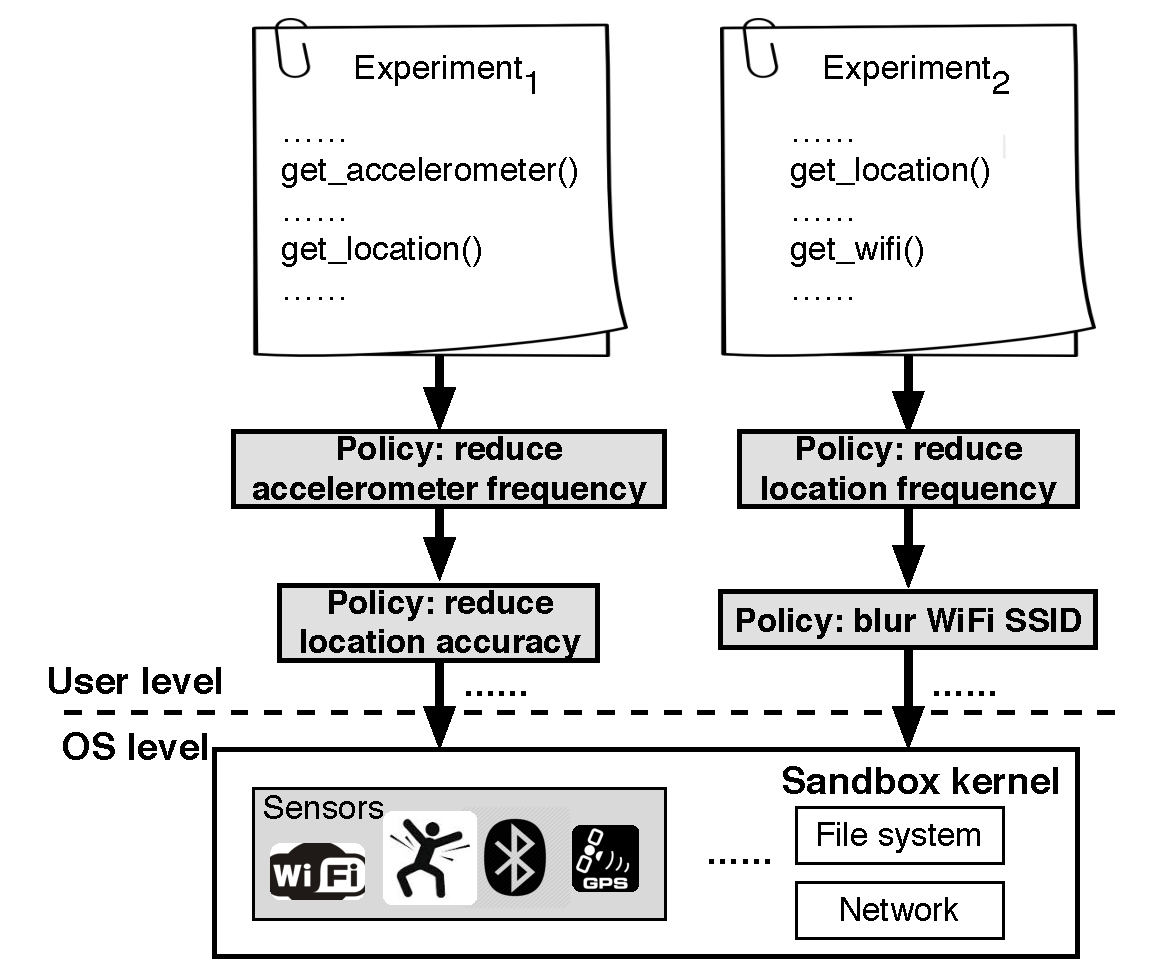
\includegraphics[width=0.7\columnwidth]{figs/blur.pdf}}
\caption{\small Policy stack demonstrating how Sensibility Testbed implements blur policies.
\label{fig-blur}}
\end{figure}


A full list of sensor API is documented at~\cite{sensor-api}. The set
of sensors range from battery, Bluetooth, and cellular, to location, WiFi, 
accelerometer, and so on. 
As such, the original Repy interface and the added sensor API together 
provide the complete \textit{OS level} sandbox kernel on a mobile 
device, as shown in Figure~\ref{fig-blur}.
